\documentclass{article}
\usepackage[utf8]{inputenc}
\usepackage{url}
\usepackage{tikz} 
\usepackage{amsmath,amssymb}
\usepackage[top=2cm,left=2cm,right=2cm,bottom=2cm]{geometry}

\title{Bayesian Methods for Machine Learning}
\author{Andrey de Aguiar Salvi}
\date{December 2020}

\newcommand{\eg}{\textit{e.g.,}}
\newcommand{\Eg}{\textit{E.g.,}}

\begin{document}

\maketitle

\section{Class 1}
Three principles:
\begin{itemize}
    \item use prior knowledge
	\item choose the answer that explains the observations the most
    \item avoid making extra assumptions
\end{itemize}
		
\subsection{Variable Independence}
\begin{equation}
	P(X, Y) = P(X)P(Y)
\end{equation}
	
\subsection{Conditional Probability}
\begin{equation}
    P(X|Y) = \frac{P(X, Y)}{P(Y)}
\end{equation}
where $P(X, Y)$ = joint probability and $P(Y)$ = marginal probability.
		
\subsection{Chain Rule}
\begin{equation}
    P(X,Y) = P(X|Y)P(Y)
\end{equation}
\begin{equation}
	P(X, Y, Z) = P(X|Y, Z)P(Y|Z)P(Z)
\end{equation}
\begin{equation}
	P(X_1, ..., X_N) = \prod_{n=1}^{N} P(X_i|X1, ..., X_{i-1})
\end{equation}
		
\subsection{Marginalization}
\begin{equation}	
	p(X) = \int_{-\inf}^{in} p(X, Y)dY
\end{equation}
		
\subsection{Bayes Theorem}

\begin{equation}	
	P(\theta|X) = \frac{P(X, \theta)}{P(X)} = \frac{P(X|\theta)P(\theta)}{P(X)}
\end{equation}
where $P(\theta|X)$ = posterior probability, $P(X|\theta)P(\theta)$ = Likelihood, and $P(X)$ = Evidence.

\section{Class 2}
\subsection{Statistic Approaches}
\begin{itemize}
    \item \textbf{Frequentist}: \begin{itemize}
        \item deterministic
		\item $\theta$ is fixed, $X$ is random
	    \item work whether data points is higher than the parameters - $|X| >> |\theta|$
		\item Train models with Maximum Likelihood: 
		\begin{equation}
		    \hat{\theta} = arg \max_\theta P(X|\theta)
		\end{equation}
	    to maximize the probability of data given the parameters
    \end{itemize}
    
    \item \textbf{Bayesing}: \begin{itemize}
        \item subjective
        \item $\theta$ is random, X is fixed (given a set of forces {$\theta$}, tossing a coin always gives the same result {$X$} )
		\item work with data on any size - $|X|$
		\item Train models with Na"(i)ve Bayes to maximize the probability of the parameters given the data
    \end{itemize}
\end{itemize}

			
\subsection{On-line learning}
Use the current mini-batch (posterior) to update parameters, and then use it as prior in the new mini-batch.

\section{Class 3}
\subsection{Bayesian Net}
Is not a bayesian neural network. The \textbf{Nodes} are random variables and the \textbf{Edges} are the direct impact.
\textbf{Model}: is the joint probability over all probabilites
\begin{equation}
    P(X_1, ..., X_N) = \prod_{n=1}^{N} P(X_i|P_a(X_i))    
\end{equation}
where $P_a(X_i)$ is the probability of the parent nodes from the Bayesian Net.
\Eg
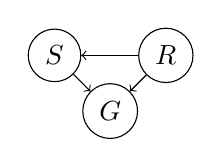
\begin{tikzpicture}[main/.style = {draw, circle}]  
    \node[main] (1) {$S$}; 
    \node[main] (2) [below right of=1] {$G$}; 
    \node[main] (3) [above right of=2] {$R$};
    \draw[->] (1) -- (2);
    \draw[->] (3) -- (1);
    \draw[->] (3) -- (2);
\end{tikzpicture} 
where R is father from G and S, S is parent from G, and the equation bellow is the respective bayesian probability
\begin{equation}
    P(S, R, G) = P(G|S, R)P(S|R)P(R)    
\end{equation}

\section{Class 5}
\subsection{Univariate Normal Distribution}
\begin{equation}
	\mathcal{N}(x|\mu, \sigma^2) = \frac{1}{\sqrt{2\pi\sigma^2}} e^{-\frac{(x - \mu)^2}{2\sigma^2}}    
\end{equation}
	
\subsection{Multivariate Normal Distribution}
\begin{equation}
    \mathcal{N}(x|\mu, \Sigma^2) = \frac{1}{\sqrt{2\pi\Sigma^2}} e^{-\frac{1}{2}(x - \mu)^T\Sigma^-1(x - \mu)}    
\end{equation}
		
\subsection{Linear Regression}
\begin{equation}
    L(w) = \sum_{i=1}^{N} (w^T x_i - y_i)^2 = ||w^T X - y|| \rightarrow \min_w
\end{equation}
\begin{equation}
    \hat{w} = arg \min_{w} L(w) 
\end{equation}
where $L$ is the loss from the bayesian net, $w$ are the weights and $X$ are the data, both are parents of $y$ (target)
\begin{equation}
    P(w, y|X) = P(y|X, w)P(w)
\end{equation}
\begin{equation}
    P(y|w, X) = \mathcal{N}(y|w^TX, \sigma^2\mathcal{I})
\end{equation}
\begin{equation}
    P(w) = \mathcal{N}(w|0, \gamma^2\mathcal{I}) 
\end{equation}
\begin{equation}
    P(w| y, x) = \frac{P(y, w|X)}{P(y|X)} \rightarrow \max_w
\end{equation}
\begin{equation}
    P(y, w|x) = \frac{P(y|x, w)}{P(w)} \rightarrow \max_w
\end{equation}

\section{Class 6 - Maximum a Posteriori}
To learn a distribution
\begin{equation}
    \theta_{MP} = arg \max_\theta P(\theta|X) = arg \max_\theta \frac{P(\theta|X)P(\theta)}{P(X)} = arg \max_\theta P(\theta|X)P(\theta)    
\end{equation}	
We eliminate the denominator from the last equation, once time it don't have $\theta$
Problems: \begin{itemize}
    \item it is not variant to reparametrization. Ex learning about a gaussian will be not usefull in sigmoid(gaussian)
	\item strange "loss function"
	\item we do not have the posteriori of $\theta$
	\item can't compute credible intervals
\end{itemize}		
			

\section{Class 7 - Conjugate Distribution}
It is a way to avoid computing the evidence ($P(X)$), which is costly. In the Bayes Probability
\begin{equation}
    P(\theta|X) = \frac{P(X|\theta)P(\theta)}{P(X)}
\end{equation}
in the likelihood, $P(X|\theta)$ is fixed by the model, $P(X)$ is fixed by the data, and $P(\theta)$ is our own choice. The prior $P(\theta)$ is conjugate to the likelihood if the prior and the posterior $P(X|\theta)$ lie in the same family distributions. 

\Eg if the prior is $P(X|\theta) = \mathcal{N}(x|\mu, \sigma^2)$ and the posterior is $P(\theta) = \mathcal{N}(\theta|m, s^2)$, thus the conjugate of posterior $P(\theta|X)$ is $\mathcal{N}(\theta|a, b^2)$.
\begin{equation}
    P(\theta|X) = \frac{P(X|\theta)P(\theta)}{P(X)} = \frac{\mathcal{N}(x|\theta, 1) \mathcal{N}(\theta|0, 1)}{P(X)}
\end{equation}
\begin{equation}
    P(\theta|X) \propto e^{-\frac{1}{2}(X - \theta)^2} e^{-\frac{1}{2}\theta^2}
\end{equation}
\begin{equation}
    P(\theta|X) \propto e^{-(\theta - \frac{X}{2})^2}
\end{equation}
\begin{equation}
    P(\theta|X) = \mathcal{N}(\theta|\frac{X}{2}, \frac{X}{2})
\end{equation}

\section{Class 8}

\subsection{Gamma Distribution}
\begin{equation}
    \Gamma(\gamma|a, b) = \frac{b^a}{\Gamma(a)} \gamma^{a-1}e^{-b\gamma}
\end{equation}
where \begin{itemize}
    \item $\gamma, a, b > 0$
    \item $\Gamma(n) = (n - 1)!$
    \item the expectation, or mean, $\mathbb{E}[\gamma] = \frac{a}{b}$
    \item $Mode[\gamma] = \frac{a-1}{b}$
    \item $Var[\gamma] = \frac{a}{b^2}$
\end{itemize}

\subsection{Precision}
\begin{equation}
    \gamma = \frac{1}{\sigma^2}
\end{equation}

If we replace the variance in the Normal Distribution to the inverse of the Precision, we get
\begin{equation}
    \mathcal{N}(x|\mu, \gamma^{-1}) = \frac{\sqrt{\gamma}}{\sqrt{2\pi}} e^{-\gamma\frac{(x - \mu)^2}{2}}    
\end{equation}
thus, the conjugate prior in respect to the precision is
\begin{equation}
    \mathcal{N}(x|\mu, \gamma^{-1}) \propto \gamma^{\frac{1}{2}}e^{-b\gamma}
\end{equation}
\begin{equation}
    P(\gamma) \propto \gamma^{a-1}e^{-b\gamma}
\end{equation}
\begin{equation}
    P(\gamma|X) = \Gamma(\gamma|a, b)
\end{equation}
then, the prior is
\begin{equation}
    P(\gamma|X) = \Gamma(\gamma|a, b) \propto  \gamma^{a-1}e^{-b\gamma}
\end{equation}
the posterior is
\begin{equation}
    P(\gamma|X) \propto P(X|\gamma)P(\gamma)
\end{equation}
dropping out all the constants, we have
\begin{equation}
    P(\gamma|X) \propto \left(\gamma^{\frac{1}{2}}e^{-\gamma \frac{(X - \theta)^2}{2}} \right) \left(\gamma^{a-1} e^{-b\gamma} \right)
\end{equation}
re-arranging the terms, we get
\begin{equation}
    P(\gamma|X) \propto \gamma^{\frac{1}{2} + a - 1}e^{-\gamma \frac{(X - \theta)^2}{2}} e^{-\gamma(b + \frac{(X - \mu)^2}{2})} 
\end{equation}
finally
\begin{equation}
    P(\gamma|X) = \Gamma(a + \frac{1}{2}, b + \frac{(X - \mu)^2}{2})
\end{equation}

\section{Class 9}
\subsection{Beta Distribution}
\begin{equation}
    \beta(X|a, b) = \frac{1}{\beta(a, b)}X^{a-1}(1 - X)^{b - 1}
\end{equation}
where:\begin{itemize}
    \item $X \in [0, 1]$
    \item $a, b > 0$
    \item \begin{equation}
        \beta(a, b) = \frac{\Gamma(a+b)}{\Gamma(a)\Gamma(b)}
    \end{equation}
    \item \begin{equation}
        \mathbb{E}[X] = \frac{a}{a+b}
    \end{equation}
    \item \begin{equation}
        Mode[X] = \frac{a-1}{a+b-2}
    \end{equation}
    \item \begin{equation}
        Var[X] = \frac{ab}{(a+b)^2(a+b-1)}
    \end{equation}
\end{itemize} 
\Eg to model a distribution with mean $0.8$ and standard deviation of $0.1$, thus $\mathbb{E}[X] = 0.8$ and $Var[X] = 0.1^2$. Consequently, a Beta distribution with $a = 12$ and $b = 3$ model it.

\subsection{Bernoulli Distribution}
The Beta distribution is the conjugate of the Bernoulli likelihood. \Eg a Bernoulli likelihood from a dataset
\begin{equation}
    P(X|\theta) = \theta^{N_1}(1-\theta)^{N_0}
\end{equation}
where $N_1$ is the number of ones in $X$ and $N_0$ the number of zeros. Thus, the Beta distribution is
\begin{equation}
    P(\theta) = \beta(\theta|a, b) \propto \theta^{a-1}(1-\theta)^{b-1}
\end{equation}
Multiplying the likelihood by the prior
\begin{equation}
    P(\theta|X) \propto P(X|\theta)P(\theta)
\end{equation}
using the before, but replacing the terms by the equivalent equations above, we have
\begin{equation}
    P(\theta|X) \propto \theta^{N_1}(1-\theta)^{N_0} \beta(\theta|a, b) \propto \theta^{a-1}(1-\theta)^{b-1}
\end{equation}
and rearranging the terms, we have
\begin{equation}
    P(\theta|X) \propto \theta^{N_1 + a - 1}(1 - \theta)^{N_0 + b - 1}
\end{equation}
and finally, recognizing the equation before as a Beta distribution, we have
\begin{equation}
    P(\theta|X) = \beta(N_1 + a, N_0 + b)
\end{equation}

\subsection{Posteriors}
\begin{itemize}
    \item Pros \begin{itemize}
        \item Exact posterior
        \item Easy for on-line learning. \Eg $P(\theta|X) = \beta(N_1 + a, N_2 + b)$
    \end{itemize}
    
    \item Cons \begin{itemize}
        \item In some cases, the conjugate prior may be inadequate
    \end{itemize}
\end{itemize}

\section{Class 10 - Latent Variable}
It is a hidden variable that you never observe. \Eg creating a dataset of a job interview, measuring the GPA, IQ, School degree, and Phone, from a first stage of the interview, and a last attribute Onsite performance, from the second interview. Traditional ML models will suffer with the missing data. Even more, probably there are some correlation between the variables, and ponder each combination will increase the number of attributes. Thus, we can link all these attributes with a latent variable, called in this example as Intelligence. We can model the problem as:
\begin{equation}
    P(X_1, X_2, X_3, X_4, X_5) = \sum_{i=1}^N P(X_1, X_2, X_3, X_4, X_5|I)P(I)
\end{equation}
where I is the latent variable. We can also simplify the problem with
\begin{equation}
    P(X_1, X_2, X_3, X_4, X_5) = \sum_{i=1}^N P(X_1|I)P(X_2|I)P(X_3|I)P(X_4|I)P(X_5|I)P(I)
\end{equation}
which breaks the table in 5 fewer tables, reduce the model complexity and improves the flexibility of the model.


\section{Class 12 - Gaussian Mixture Model (GMM)}
It is a model of soft clustering with $N$ gaussian's can be described as
\begin{equation}
    P(X|\theta) = \pi_1\mathcal{N}(\mu_1, \Sigma_1) + \pi_2\mathcal{N}(\mu_2, \Sigma_2) + ... + \pi_N\mathcal{N}(\mu_N, \Sigma_N)
\end{equation}
where the $\theta$ weight matrix is 
\begin{equation}
    \theta = \{\pi_1, \pi_2, ..., \pi_N, \mu_1, \mu_2, ..., \mu_N, \Sigma_1, \Sigma_2, ..., \Sigma_N\}
\end{equation}
To goal of the train is
\begin{equation}
    \max_\theta P(X|\theta) = \prod_{i=1}^N P(X_1|\theta) = \prod_{i=1}^N \left( pi_1\mathcal{N}(\mu_1, \Sigma_1) + ... \right)
\end{equation}
By definition, the covariance matrix $\Sigma_k \succ 0$, once time we need to compute $\Sigma^{-1}$. Otherwise, we will have divisions by zero.

\section{Class 13 - Training a GMM}
Assuming that our data points $X$ was generated by a latent variable $t$. Thus, the probability of a point to belongs to the class $c$ given the parameters $\theta$ is
\begin{equation}
    P(t = c|\theta) = \pi_c
\end{equation}
and 
\begin{equation}
    P(X|t = c, \theta) = \mathcal{N}(X, \mu_c, \Sigma_c)
\end{equation}
Marginalizing the latent variable, we have
\begin{equation}
    P(X|\theta) = \sum_{c=1}^N P(X|t = c, \theta)P(t = c|\theta)
\end{equation}
which is the summation of the likelihood times the prior, and is exactly the same as the first equation, but ignoring the latent variable.

Training a GMM, if we have hard-labels of the points, it is a easy problem: we just need to compute the mean and standard deviation of each cluster. In the opposite side, if we have the parameters (consequently the gaussians), thus we can estimate the source ($P(t = 1|X, \theta) = \frac{P(X|t = 1, \theta)P(t = 1|\theta)}{Z}$), which is the joint probability (the likelihood times the prior). The problem of train a GMM is a Chicken and Egg problem:
\begin{itemize}
    \item Need gaussian parameters ($\theta$) to estimate the source (soft-labels)
    \item Need sources to estimate the gaussian parameters
\end{itemize}

\section{Class 14 - EM GMM}
\begin{enumerate}
    \item Start with $N$ randomly placed gaussians parameters $\theta$
    \item Until convergence: \begin{enumerate}
        \item For each point $X_i$, compute $P(t = c|X_i, \theta)$
        \item Update gaussian parameters $\theta$ to fit points assigned to them
    \end{enumerate}
\end{enumerate}

\begin{itemize}
    \item EM can train GMM faster than Stochastic Gradient Descent
    \item EM suffers from local maxima (the exact solution is NP-Hard)
\end{itemize}

\section{Class 15}
\subsection{Concavity}
A function is concave if its second derivative is negative, or, if 
\begin{equation}
    f(\alpha a + (1 - \alpha)b) \geq \alpha f(a) + (1 - \alpha)f(b)
\end{equation}
where $0 \leq \alpha \leq 1$. The Figure \ref{fig:inequality} shows an \eg
\begin{figure}[!t]
    \centering
    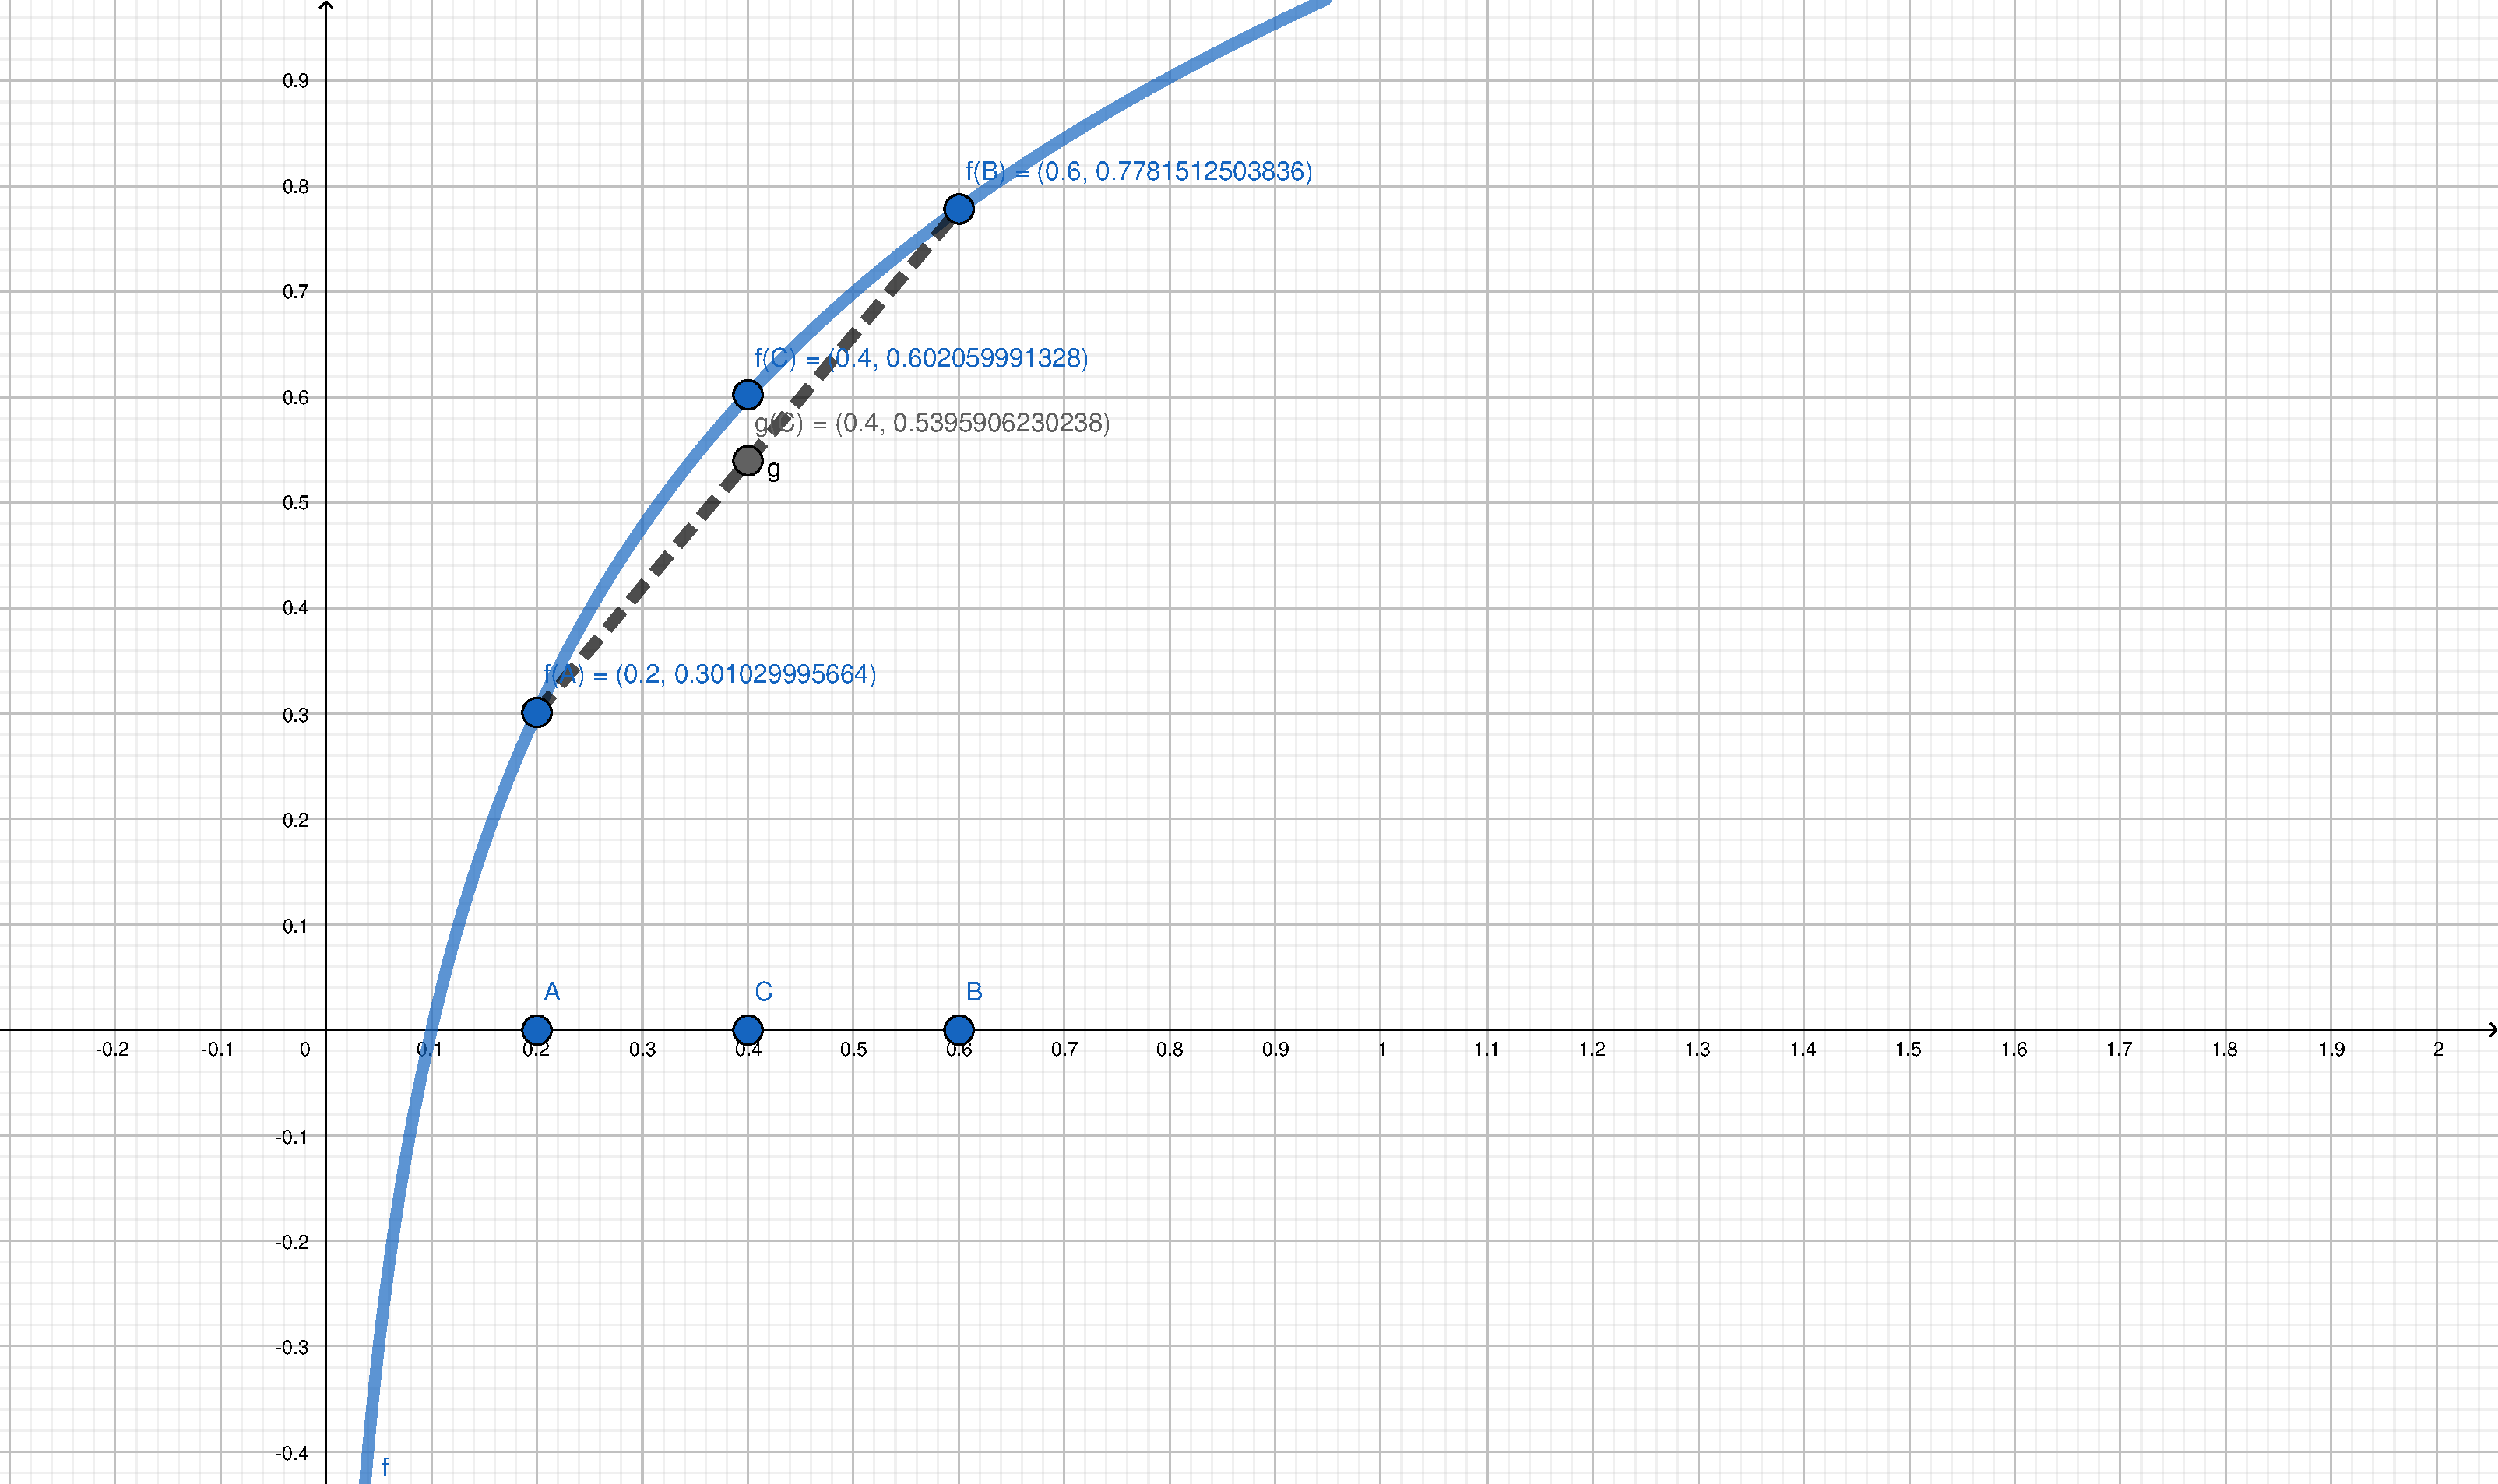
\includegraphics[width=\textwidth]{geogebra.pdf}
    \caption{Showing the inequality from the equation. The equation from the right inequality side, which generates the straight segment, we call as G(x).}
    \label{fig:inequality}
\end{figure}

\subsection{Jensen's inequality} 
Generalizing the concavity for any point, we have 
\begin{equation}
    f(\mathbb{E}_{p(t)t}) \geq \mathbb{E}_{p(t)}f(t)
\end{equation}

\subsection{Kullback-Leibler Divergence} 
It is a way to measure the difference between two probabilistic functions.
\begin{equation}
    \mathcal{K}\mathcal{L}(p || q) = \int q(x) \log \frac{q(x)}{p(x)} dx
\end{equation}
Properties: \begin{enumerate}
    \item \begin{equation}
        \mathcal{K}\mathcal{L}(p || q) \neq \mathcal{K}\mathcal{L}(q || p)
    \end{equation}
    \item \begin{equation}
        \mathcal{K}\mathcal{L}(q || q) = 0
    \end{equation}
    \item \begin{equation}
        \mathcal{K}\mathcal{L}(p || q) > 1
    \end{equation}
\textcolor{red}{Proof}
\begin{equation}
    - \mathcal{K}\mathcal{L}(p || q) = \mathbb{E}_q \left(-\log \frac{q}{p} \right) = \mathbb{E}_q \left(\log \frac{p}{q} \right)
\end{equation}
\begin{equation}
    \leq \log \left(\mathbb{E}_q \frac{p}{q} \right) = \log \int q(x) \frac{p(x)}{q(x)}dx = 0
\end{equation}
\end{enumerate}

\section{Class 16 - Expectation Maximization}
Using the log for mathematical conveniences, we want to
\begin{equation}
    \max_\theta \log (P(X|\theta)) = \log \left( \prod_{i=1}^N p(x_i|\theta) \right)
\end{equation}
with the log properties, we have
\begin{equation}
    \max_\theta \log (P(X|\theta)) = \log \left( \sum_{i=1}^N \log (p(x_i|\theta)) \right)
\end{equation}
The probability $\log (p(x|\theta))$ is
\begin{equation}
    \log (p(x|\theta)) = \log \left( \sum_{i=1}^N \log (p(x_i|\theta)) \right)
\end{equation}
which we can change the marginal likelihood of the data object $x_i$ by the definition, resulting in
\begin{equation}
    = \sum_{i=1}^N \log \left( \sum_{c=1}^C p(x_i, t_i = c| \theta) \right)
\end{equation}
with the Jensen's inequality, we have
\begin{equation}
    = \sum_{i=1}^N \log \left( \sum_{c=1}^C p(x_i, t_i = c| \theta) \right) \geq \mathcal{L}(\theta)
\end{equation}
which means that instead of maximize the original marginal log likelihood, we will maximize a lower bound instead, which is more easy to maximize. Multiplying a dividing a term by the same value, we don't change the function. So, for convenience, we have
\begin{equation}
    = \sum_{i=1}^N \log \left( \sum_{c=1}^C \frac{\textcolor{blue}{q(t_i = c)}}{\textcolor{orange}{q(t_i = c)}} \textcolor{orange}{p(x_i, t_i = c| \theta)} \right) 
\end{equation}
rewriting, what we have is the Jensen's inequality, in this equation
\begin{equation}
    \log \left( \sum_c \textcolor{blue}{\alpha_c}\textcolor{orange}{\upsilon_c} \right) = \sum_c \left( \log \textcolor{blue}{\alpha_c}(\textcolor{orange}{\upsilon_c}) \right)
\end{equation}
applying the logarithm properties from the Jensen's inequality, we rebuild the function to
\begin{equation}
    \geq \sum_{i=1}^N \sum_{c=1}^C \left(\textcolor{blue}{q(t_i = c)} \log\frac{\textcolor{orange}{p(x_i, t_i = c| \theta}}{\textcolor{orange}{q(t_i = c)}}  \right)
\end{equation}
\begin{equation}
    = \mathcal{L}(\theta, q)
\end{equation}
Graphically, we are changing the loss as we change the value of $q$, as in Figure \ref{fig:L}.
\begin{figure}
    \centering
    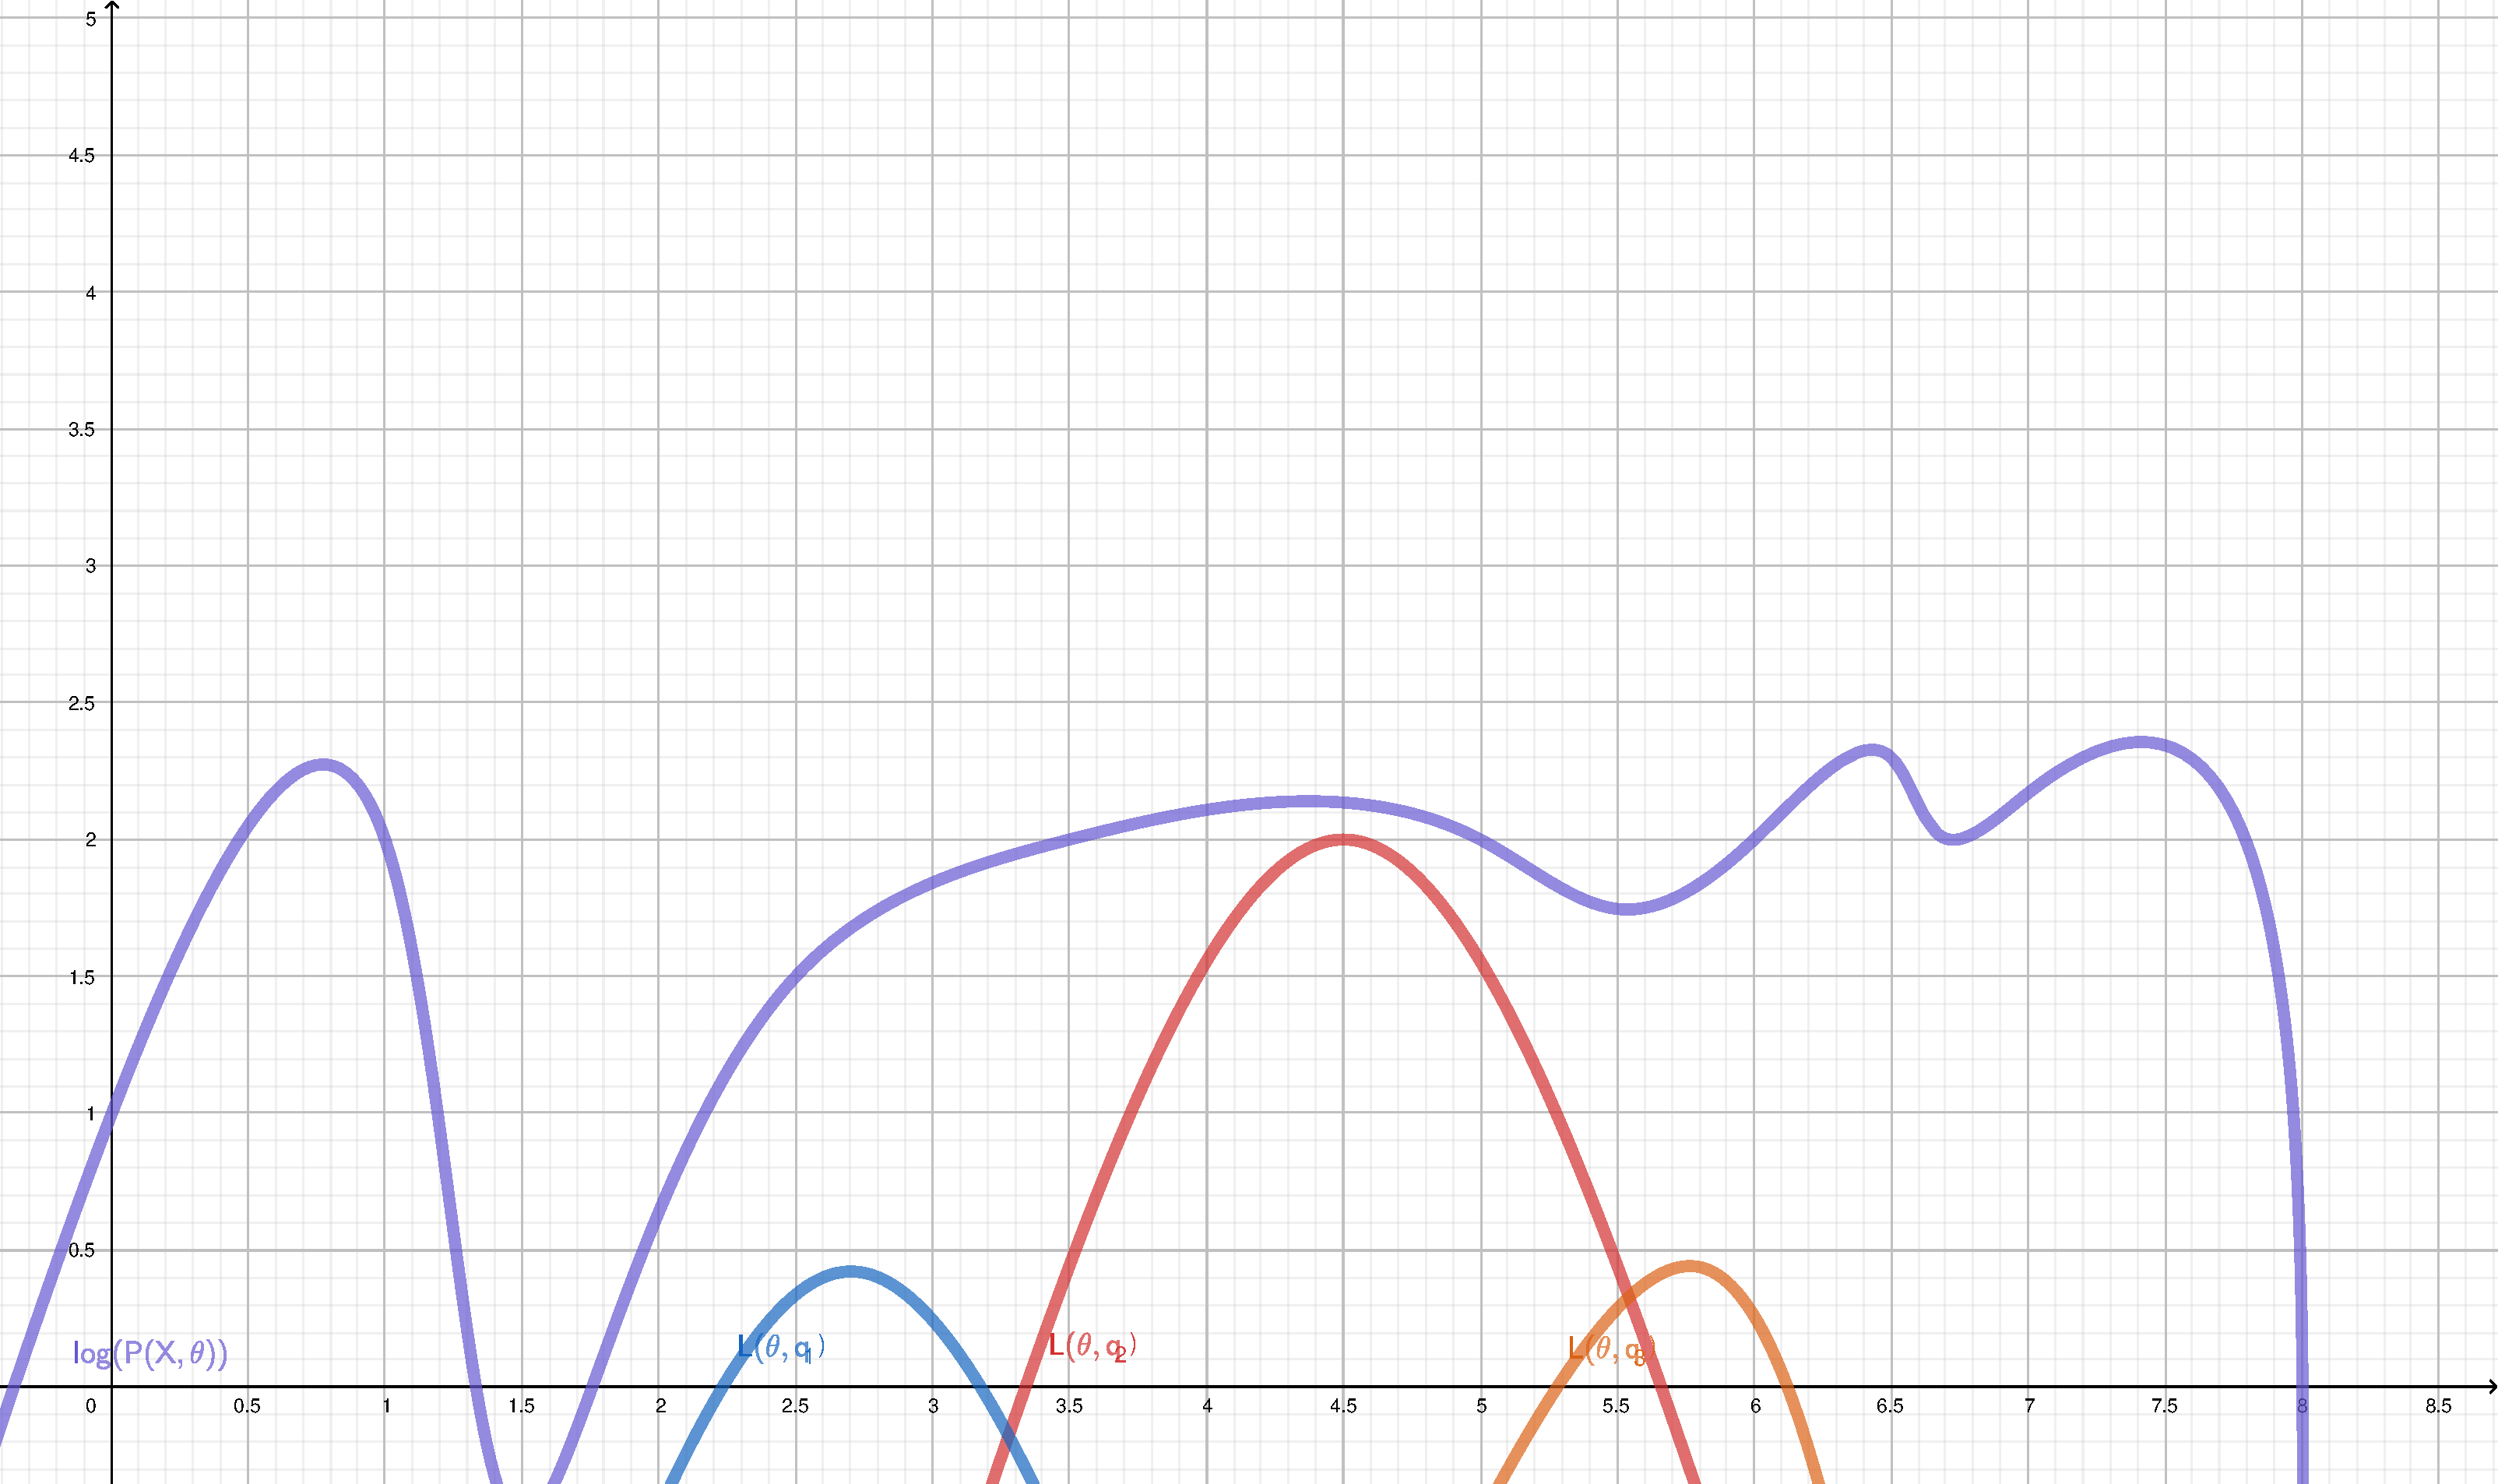
\includegraphics[width=\textwidth]{L.pdf}
    \caption{Loss from the General Form of Expectation of Maximization, changing $q$ value. $\theta$ is the x-axis.}
    \label{fig:L}
\end{figure}
In practice, fixing $q$ we have a new loss $\mathcal{L}$, as the blue curve in figure, which tends to have an global optimum point similar to a local optimum point in the original curve, the purple. In the next $q$ step, we have another curve. Repeating iteratively, these variational lower-bound curves tends to lead $\theta$ to the global optimal point from the original curve.

Summarizing:
\begin{itemize}
    \item $\log p(X|\theta) \geq \mathcal{L}(\theta, q)$ for any $q$, where $\mathcal{L}(\theta, q)$ is the variational lower bound
    \item \textbf{E-step} \begin{equation}
        q^{k+1} = arg \max_q \mathcal{L}(\theta^k, q)
    \end{equation}
    \item \textbf{M-step} \begin{equation}
        \theta^{k+1} = arg \max_\theta \mathcal{L}(\theta, q^{k+1})
    \end{equation}
\end{itemize}

\section{Class 17 - E Step}
Fixing $\theta$ and maximizing $\mathcal{L}$, which is a log likelihood, changing $q$, which is a distribution
\begin{equation}
    \max_q \mathcal{L}(\theta^k, q)
\end{equation}
as in Figure \ref{fig:L}, we want to minimize the gap between the purple curve, the real log likelihood $\log P(X|\theta)$, and some another curve, which is fixed the current lower bound at step $k$. We can describe the gap as
\begin{equation}
    gap = \log P(X|\theta) - \mathcal{L}(\theta^k, q)
\end{equation}
which is equal to
\begin{equation}
    = \sum_{i=1}^N \log P(X_i|\theta) - \sum_{i=1}^N \sum_{c=1}^C q(t_i = c) \log \frac{P(X_i, t_i = c|\theta)}{q(t_i = c)}
\end{equation}
rearranging the summations, we have
\begin{equation}
    = \sum_{i=1}^N \left( \log P(X_i|\theta) * \sum_{c=1}^N q(t_i = c) - \sum_{c=1}^C q(t_i = c) \log \frac{P(X_i, t_i = c|\theta)}{q(t_i = c)} \right)
\end{equation}
but $\sum_{c=1}^N q(t_i = c)$ is the summation of the probabilities of all the classes, which is always $1$. As the two inner summations have this element, we can rearrange the equation, giving
\begin{equation}
    = \sum_{i=1}^N \sum_{c=1}^N q(t_i = c) \left( \log P(X_i|\theta) - \log \frac{P(X_i, t_i = c|\theta)}{q(t_i = c)} \right)
\end{equation}
and using the logarithm properties of division of terms, we have
\begin{equation}
    = \sum_{i=1}^N \sum_{c=1}^N q(t_i = c) \left( \log \frac{P(X_i|\theta) q(t_i = c)}{P(X_i, t_i = c|\theta)} \right)
\end{equation}
by some bayesian rules, $P(X_i, t_i = c|\theta) = P(t_i = c|X_i, \theta)P(X_i|\theta)$, replacing the terms, we can simplify the $P(X_i|\theta)$ in the numerator and denominator, giving 
\begin{equation}
    = \sum_{i=1}^N \sum_{c=1}^N q(t_i = c) \left( \log \frac{q(t_i = c)}{P(t_i = c|X_i, \theta)} \right)
\end{equation}
where the inner summation is exactly the Kullback-Leibler Divergence $\mathcal{KL}\left(q(t_i||P(t_i|X_i, \theta)\right)$. Our final equation is
\begin{equation}
    gap = \sum_{i=1}^N \mathcal{KL}\left(q(t_i||P(t_i|X_i, \theta)\right)
\end{equation}
As we want to maximize the lower bound $\mathcal{L}$, we want to minimize the difference gived by the first gap equation, which means minimize the summation of the Kullback-Leibler Divergence.

\section{Class 18 - M Step}

\section{Class 18 - M Step}
We want to maximize the lower-bound log likelihood, as discussed in class 16 after rebuild the equation in a Jensen's inequality, with the following equation
\begin{equation}
    \mathcal{L}(\theta, q) = \sum_{i=1}^N \sum_{c=1}^N q(t_i = c) log \frac{P(X_i, t_i = c|\theta)}{q(t_i = c)}
\end{equation}
but now, in terms of $\theta$. With the division logarithm property, we can transform to the following equation to
\begin{equation}
    \mathcal{L}(\theta, q) = \sum_{i=1}^N \sum_{c=1}^N q(t_i = c) log P(X_i, t_i = c|\theta) - \sum_{i=1}^N \sum_{c=1}^N q(t_i = c) log q(t_i = c)
\end{equation}
but, as we can maximize in terms of $\theta$, and the second term haven't $\theta$, we can throw this term away, which results in
\begin{equation}
    \mathbb{E}_q \log P(X, T|\theta) + const
\end{equation}
which usually is a concave function, so it is easy to maximize. The goal in the M-step is

\subsection{Summarising Expectation Maximization}
E-step
\begin{equation}
    q^{k+1} = arg \min_q \mathcal{KL}[q(T) || P(T|X, \theta^k)] \Leftrightarrow q^{k+1}(t_i) = p(t_i|x_i, \theta^k)
\end{equation}
M-step
\begin{equation}
    \theta^{k+1} = arg \max_\theta \mathbb{E}_{q^{k+1}} \log P(X, T|\theta^k)
\end{equation}

\section{Class 19 - E step example}
Imagine a dataset with three values: $1, 2,$ and $3$, with $N_1 = 30, N_2 = 20$, and $N_3 = 60$, respectively. Threre are two gaussians to fit the data, parametrized by the parameters $\alpha$, $\beta$, and $\gamma$. The probability function is $P(x_i) = \gamma P_1(x_i) + (1 - \gamma)P_2(x_i)$. The following table gives the probability distribution to each value accordingly to each $P_n$:
\begin{table}[h]
    \centering
    \begin{tabular}{cccc}
         &  $1$ & $2$ & $3$ \\
         $P_1$ & $\alpha$ & $1 - \alpha$ & $0$ \\
         $P_1$ & $0$ & $1 - \beta$ & $\beta$ 
    \end{tabular}
    \caption{Probabilities to sample the values $1, 2$, and $3$ with the probability models $P_1$ and $P_2$.}
    \label{tab:EM_ex}
\end{table}
where $\alpha_0 = \beta_0 = \gamma_0 = 0.5$. Using the latent variable $t$ we have
\begin{equation}
    P(t_i = 1) = \gamma 
\end{equation}
\begin{equation}
    P(x_i|t_i = 2) = P_2(x_i)
\end{equation}
By definition, $q(t_i) = P(t_i = c|x_i)$, and $P(X|Y) = \frac{P(Y|X)P(Y)}{P(X)}$. Changing the terms of this equation by the values given by the example, we have
\begin{equation}
    q(t_i = 1) = P(t_i = 1|x_i = 1) = \frac{P(x_i = 1|t_i = 1)P(t_i = 1)}{P(x_i = 1|t_i = 1)P(t_i = 1) + P(x_i = 2|t_i = 2)P(t_i = 2)}
\end{equation}
looking for Table \ref{tab:EM_ex}, we have
\begin{equation}
    = \frac{\alpha \gamma}{\alpha \gamma + 0(1 - \alpha)} = 1
\end{equation}
and for $t = 2$
\begin{equation}
    = \frac{(1- \alpha) \gamma}{(1 - \alpha) \gamma + (1 - \beta)(1 - \gamma)} = \frac{0.5*0.5}{0.5*0.5 + 0.5*0.5} = 0.5
\end{equation}

\section{Class 20 - M step example}
Following the example, we have $N_1 = 30, N_2 = 20$, $\alpha_0 = \beta_0 = \gamma_0 = 0.5$, $P(x_i) = \gamma P_1(x_i) + (1 - \gamma)P_2(x_i)$, the Table \ref{tab:EM_ex} with the probabilities, and we discover in E step that
\begin{equation}
    q(t_i = 1) = P(t_i = 1|x_i) = \begin{cases}
        1, & x_i = 1 \\
        0.5, & x_i = 2\\
        0, & x_i = 3\\ 
    \end{cases}
    \label{eq:cases_EM}
\end{equation}
and $q(t_i = 2) = 1 - q(t_i = 1)$. By definition, we want a maximization with 
\begin{equation}
    \max_{\alpha, \beta, \gamma} \sum_{i=1}^N \mathbb{E}_{q(t_i)} \log p(x_i|t_i)p(t_i) = \sum_{i=1}^N q(t_i = 1) \log(p(x_i|t_i = 1))\gamma + \sum_{i=1}^N q(t_i = 2) \log(p_2(x_i))(1 - \gamma)
\end{equation}
Changing the constants by the values, we have
\begin{equation}
    = 30 P(t_i = 1|x_i = 1) \log(\alpha)\gamma + 20*0.5 \log(1 - \alpha)\gamma + 60*0*\log0 + 20*0.5 \log(1 - \beta)(1 - \gamma) + 60*1*\log(\beta)(1 - \gamma)
\end{equation}
as $P(t_i = 1|x_i = 1) = 1$ and other terms zeroed, we have
\begin{equation}
    30 \log\alpha + 1 \log(1 - \alpha) + const(\alpha)
\end{equation}
which is the problem that we want to maximize. Using the gradient (deriving the logs), we have
\begin{equation}
    30\frac{1}{\alpha} + 10\frac{1*(-1)}{1 - \alpha} = 0 \rightarrow \frac{30}{\alpha} = \frac{10}{1 - \alpha} \rightarrow 30 - 30\alpha = 10\alpha \rightarrow 40\alpha = 30 \rightarrow \alpha = \frac{3}{4} = 0.75
\end{equation}
and finally, $\beta = \frac{6}{7}$ and $\gamma = \frac{4}{11}$.

\section{Class 22 - General EM for GMM}
\begin{enumerate}
    \item E-step \begin{itemize}
        \item EM: for each point, compute $q(t_i) = p(t_i|x_i, \theta)$
        \item GMM: equally, compute $p(t_i|x_i, \theta)$
    \end{itemize}
    \item M-step \begin{itemize}
        \item EM: update parameters to maximize $\max_\theta \mathbb{E}_q \log p(X, T|\theta)$
        \item GMM: update Gaussian parameters to fit points assigned to them $\mu_i = \frac{\sum_i p(t_i = 1| x_i, \theta)x_i}{\sum_i p(t_i = 1| x_i, \theta)}$. \Eg
        \begin{equation}
            \max_\theta \mathbb{E}_q \log p(X, T|\theta) = \sum_{i=1}^N \sum_{c=1}^C q(t_i = c) \log \left(
            \frac{1}{z} e^{-\frac{(x_i-\mu_c)^2}{2\sigma_c^2}}\pi_c
            \right)
        \end{equation}
        \begin{equation}
            = \sum_{i=1}^N \sum_{c=1}^C q(t_i = c) \log(\frac{\pi_c}{z}) - -\frac{(x_i-\mu_c)^2}{2\sigma_c^2}
        \end{equation}
        and deriving it in respect to the first Gaussian, which uses $\mu_1$, we have
        \begin{equation}
            \frac{\partial...}{\partial_{\mu_c}} = \sum_{i=1}^N q(t_i = 1) (0 - \frac{2(x_i - \mu_{i=1})(-1)}{2\sigma_{c=1}^2})
        \end{equation}
        multiplying the term by $\sigma_{c=1}^2$ to eliminate the term in the denominator, and setting equal to zero (once time the lower bound log likelihood is a concave curve, and the derivative zero is in the highest point), we have
        \begin{equation}
            = \sum_{i=1}^N q(t_i = 1)x_i - \sum_{i=1}^N q(t_i = 1)\mu_{i=1} = 0
        \end{equation}
        \begin{equation}
            \mu_1 = \frac{\sum_{i=1}^N q(t_i = 1)x_i}{\sum_{i=1}^N q(t_i = 1)}
        \end{equation}
        and consequently, 
        \begin{equation}
            \sigma_c^2 = \frac{\sum_{i=1}^N q(t_i = c)(x_i-\mu_c)}{\sum_{i=1}^N q(t_i = c)}
        \end{equation}
        where $\mu_c$ here is the new $\mu$ computed by the previous one equation. For the gaussian ponder $\pi$, we have to ensure that $\pi_c > 0$ and $\sum_{c=1}^C \pi_c = 1$. We can update $\pi$ with the following equation
        \begin{equation}
            \pi_c = \frac{\sum_{i=1}^N q(t_i = c)}{N}
        \end{equation}
    \end{itemize}
\end{enumerate}

\section{Class 23}
\subsection{K-Means from GMM Perspective}
In GMM, if we fix the covariances to be identical, $\Sigma_c = \mathcal{I}$, and fix the weights of each gaussian to be uniform, $\pi_c = \frac{1}{N Gaussians}$, thus, the conditional probability is
\begin{equation}
    p(x_i|t_i = c, \theta) = \frac{1}{Z} e^{-0.5||x_i - \mu_c||^2}
\end{equation}
which is a weighted euclidean distance between the data and the centroid. Thus, we prove that the K-Means is a special case of the GMM.

\subsection{K-Means from EM perspective}
The $q(t)$ is approximated by a delta function, which binaries the probabilities
\begin{equation}
    q^{k+1}(t_i) = \begin{cases}
    1, & t_i = c_i\\
    0, & otherwise\\
    \end{cases}
\end{equation}
then, the \textbf{E-step} turns
\begin{equation}
    c_i = arg \max_c p(t_i = c|x_i, \theta)
\end{equation}
where the probability $p(t_i = c|x_i, \theta)$ is 
\begin{equation}
    p(t_i = c|x_i, \theta) = \frac{1}{Z}p(x_i|t_i, \theta)p(t_i\theta)
\end{equation}
\begin{equation}
    = \frac{1}{Z}e^{-0.5||x_i - \mu_c||^2}\pi_c
\end{equation}
as $\frac{1}{Z}$ and $\pi_c$ does not depend on $c$, we can throw it away. Then, the \textbf{E-step} becomes to
\begin{equation}
    c_i = arg \max_c p(t_i = c|x_i, \theta) = arg \min_c ||x_i - \mu_c||^2
\end{equation}
which is the Euclidean distance used in K-Means.

\section{Class 24 - K-Means from EM perspective}
The \textbf{M-step} is
\begin{equation}
    \max_\mu \sum_{i=1}^N \mathbb{E}_{q(t_i)} \log(p(x_i, t_i|\mu))
\end{equation}
where $\mu$ is relative to the parameters from the original equation. As $q(t_i)$ is restricted, as the equation bellow,
\begin{equation}
    q(t_i) = \begin{cases}
    1, & t_i = c_i^*\\
    0, & t_i \neq c_i^*\\
    \end{cases}
\end{equation}
and do not contribute in the equations, we can rewrite the $\mu$ update to
\begin{equation}
    \mu_c = \frac{\sum_{i=1}^N q(t_i = c)x_i}{\sum_{i=1}^N q(t_i = c)} = \frac{\sum_{i: c_i^*=c_i}^N x_i}{N i: c_i^*=c_i }
\end{equation}
which is exactly the mean of the classified points, as the K-Means do.

\section{Class 25 - Probabilistic Principal Component Analysis (PPCA)}
We can model a PCA as a probabilistic model using latent variables. Thus, we can threat missing data. Imaging a PCA reducing two dimensions to the dimension $t$. Thus, threating as a latent variable, we have
\begin{equation}
    p(t_i) = \mathcal{N}(0, I)
\end{equation}
and the points that precisely overlaps the PCA curve are computed by
\begin{equation}
    x_i = \mathcal{W}t_i + b
\end{equation}
while the original data from the dataset can be estimated as 
\begin{equation}
    x_i = \mathcal{W}t_i + b + \epsilon_i
\end{equation}
where $\sigma_i$ is a random noise with $\epsilon_i ~ \mathcal{N}(0, \Sigma$. probabilistically, we have
\begin{equation}
    p(x_i|t_i, \theta) = \mathcal{N}(\mathcal{W}t_i + b, \Sigma)
\end{equation}
As we have continuous variables, we need the Marginalization to train the model
\begin{equation}
    \max_\theta p(X|\theta) = \prod_{i=1}^N p(x_i|\theta) = \prod_{i=1}^N \int p(x_i|t_i, \theta)p(t_i)dt_i
\end{equation}
which is intractable, as the integral means summing all the points. Applying a conjugacy in the integral, resulting in $\mathcal{N}(\mu_i, \Sigma_i)$, we can treat this problem training with Expectation Maximization.

\section{Class 26 - EM for PPCA}
\textbf{E-step}
\begin{equation}
    q(t_i) = p(t_i|x_i, \theta) = \frac{p(x_i|t_i, \theta)p(t_i)}{Z} = \mathcal{N}(\hat{\mu_i}), \hat{\Sigma_i}
\end{equation}
\textbf{M-step}
\begin{equation}
    \max_\theta \mathbb{E}_{q(T)} \sum_i \log\left(p(x_i|t_i, \theta)p(t_i) \right) = \sum_i \mathbb{E}_{q(t_i)} \log\left( \frac{1}{Z}e^{...}e^{...} \right)
\end{equation}
as $\frac{1}{Z}$ not depends of $t_i$, and with the logarithm property of log multiplication is equal to the sum of the logs, we rewrite to
\begin{equation}
    = \sum_i \log(\frac{1}{Z}) + \sum_i \mathbb{E}_{q(t_i)} \log\left(e^{...}e^{...} \right)
\end{equation}
\begin{equation}
    = \sum_i \log(\frac{1}{Z}) + \sum_i \mathbb{E}_{q(t_i)} \log\left(exp\left(-\frac{(x - \mathcal{W}t_i - b)^2}{2\sigma^2}\right) exp\left(-\frac{t_i^2}{2}\right) \right)
\end{equation}
where all the log term is similar to $at_i^2 + ct_i + d$.

\section{Class 27 - Inference Approximation}
In some cases, the we can approximate a distribution by another, as the marginal probability can be hard to compute. We can, \eg, train a neural network to learn a distribution, switching the marginal probability by a constant normalization
\begin{equation}
    p^*(z) = p(z|X) = \frac{p(X|z)p(Z)}{p(X)} = \frac{\hat{p}(Z)}{Z}
\end{equation}
In this manner, we need to minimize the $\mathcal{KL}$-Divergence
\begin{equation}
    \mathcal{KL}[q(z)||\frac{\hat{p}(Z)}{Z}] = \int q(z)\log\left(\frac{q(z)}{\hat{p}(Z)/Z}\right)dz = \int q(z)\log\left(\frac{q(z)}{\hat{p}(Z)}\right)dz + \int q(z) \log Z dz 
\end{equation}
\begin{equation}
    \mathcal{KL}[q(z)||\hat{p}(Z)] + \log Z
\end{equation}
as $\log Z$ is a constant, we have
\begin{equation}
    \mathcal{KL}[q(z)||\hat{p}(Z)] \rightarrow \min_z
\end{equation}

\section{Class 28 - Mean Field}
\begin{enumerate}
    \item Select a family of distributions $\mathcal{Q}$ as a variational inference
    \begin{equation}
        \mathcal{Q} = {q|q(z) = \prod_{i=1}^d q_i(z)}
    \end{equation}
    which is a set of all distributions that have factorized over the dimensions of the latent variables.
    \item optimize to find the best approximation $q(Z)$ of $\hat{p}(Z)$
    \begin{equation}
        \mathcal{KL}[q(z)||\hat{p}(Z)] \rightarrow \min_{q \in \mathcal{Q}}
    \end{equation}
\end{enumerate}
\Eg, factorizing a distribution of two variables to a multiplication of two distributions: $p^*(z_1, z_2) \approx q_1(z_1)q_2(z_2)$, where $p^*$ is the real distribution. Imaging that $p^*(z_1, z_2) = \mathcal{N}(0, \Sigma)$. Thus, we have $q_1(z_1)q_2(z_2) = \mathcal{N}(0, \begin{pmatrix}
    \sigma_1^2 & 0\\
    0 & \sigma_2^2
\end{pmatrix})$. Then, optimize the $\mathcal{KL}$-Divergence for each distribution,
\begin{equation}
    \mathcal{KL}(\prod_i^d q_i||p^*) \rightarrow \min_q
\end{equation}
and the $\mathcal{KL}$-Divergence is
\begin{equation}
    = \int\prod_i^d \log\left(\frac{\prod_i^d q_i}{p^*} \right)dz = \sum_i^d \int\prod_j^d \log(q_i)dz - \int\prod_j^d \log(p^*)dz
\end{equation}
where, for a specific distribution $k$, we eliminate the first summation and generate 
\begin{equation}
    = \int\prod_j^d \log(q_k)dz + \sum_{i\neq k}^d \int\prod_j^d \log(q_i)dz - \int\prod_j^d \log(p^*)dz
\end{equation}
but, some therms are constants in relation to $q(z)$ and its respective integrals are equal to $1$. \Eg, the first integral can be decomposed to
\begin{equation}
    \int\prod_j^d \log(q_k)dz = \int q_k\log(q_k)\left[\int\prod_{j\neq k}^d \log(q_j)dz_{\neq k} \right]dz_k = \int q_k\log(q_k) dz_k
\end{equation}
The second integral not depends on $k$, and thus it is constant. Rewriting, we have
\begin{equation}
    \int\prod_i^d \log\left(\frac{\prod_i^d q_i}{p^*} \right)dz = \int q_k\log(q_k) dz_k - \int q_k \left[\prod_{j\neq k}^d q_j \log(p^*) dz_{\neq k}\right]dz_k
\end{equation}
grouping the similar term $q_k$, we have
\begin{equation}
    = \int q_k \left[\log(q_k) dz_k - \int \prod_{j\neq k}^d q_j \log(p^*) dz_{\neq k}\right] dz_k
\end{equation}
and the term with the productory is the expectation, $h(z_k) = \mathbb{E}_{q_{-k}}\log p^* = prod_{j\neq k}^d q_j \log(p^*) dz_{\neq k}$. If we rewrite $h(z)$ as $t(z_k) = \frac{e^{h(z_k)}}{\int e^{h(z_k)}dz_k}$, we can rewrite the last equation to a $\mathcal{KL}$-Divergence
\begin{equation}
    = \int q_k \log\left(\frac{q_k}{t}\right)dz_k + const = \mathcal{KL}(q_k||t) \rightarrow \min
\end{equation}
as we want to zero the $\mathcal{KL}$-Divergence, then
\begin{equation}
    q_k = t \rightarrow \log q_k = \mathbb{E}_{q_{-k}} \log p^* + const
\end{equation}

\end{document}
